\documentclass{article}
\usepackage[a4paper, total={7in, 10in}]{geometry}
\usepackage{fontspec} 
\usepackage{xeCJK} 
\setCJKmainfont{標楷體}
\setmainfont{Times New Roman}
\XeTeXlinebreaklocale “zh” 
\XeTeXlinebreakskip = 0pt plus 1pt
\usepackage{graphicx}
\usepackage{float}
\usepackage{xcolor}
\usepackage[linesnumbered,ruled,vlined]{algorithm2e}
\usepackage{mathtools}
\usepackage{amsmath} 
\usepackage{subfigure}  




\newcommand\mycommfont[1]{\footnotesize\ttfamily\textcolor{blue}{#1}}
\SetCommentSty{mycommfont}

\SetKwInput{KwInput}{Input}                % Set the Input
\SetKwInput{KwOutput}{Output}              % set the Output

\title{Self-Driving Cars}
\author{309611087 洪得瑜}
\date{2022 10/27} 

\begin{document}
\maketitle

\section{Kalman Filter Impluement in Real Data}
\begin{figure}[H]
\centering
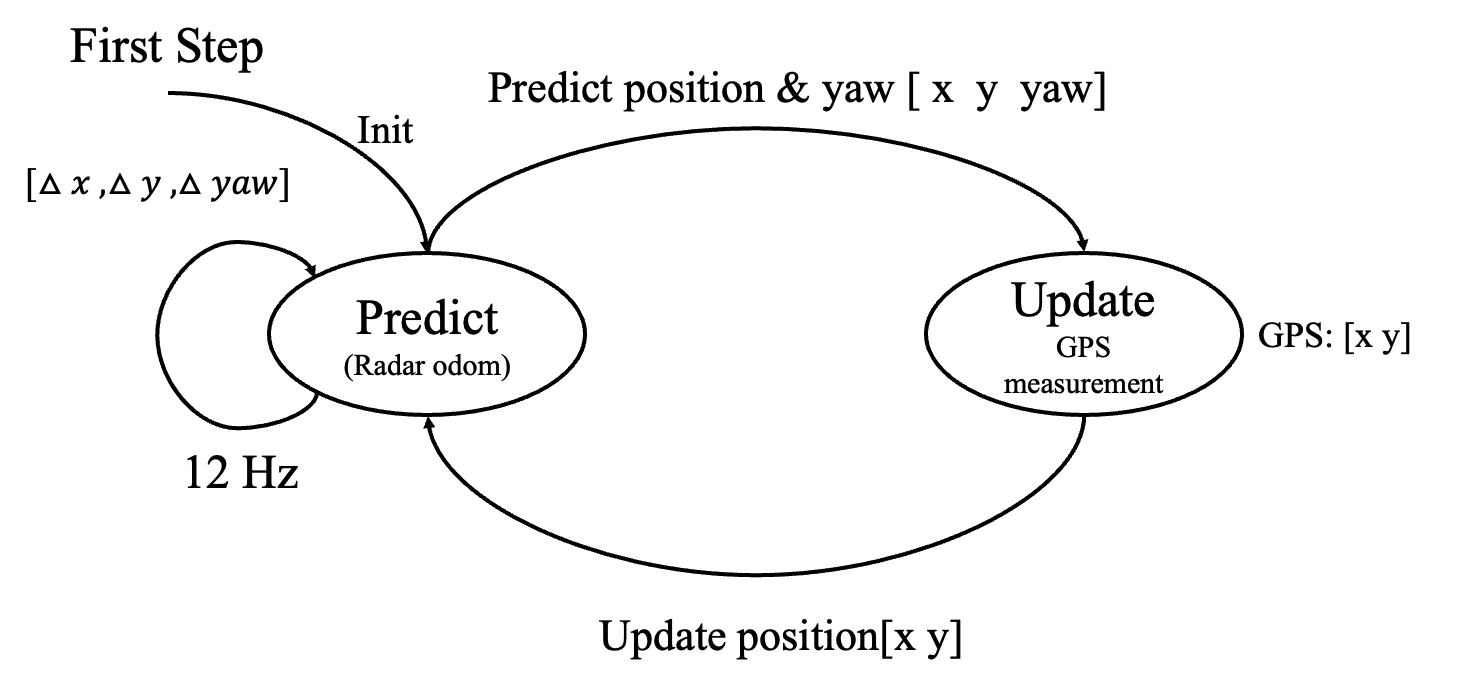
\includegraphics[scale = 0.2]{./state.png}
\end{figure}

\subsection{Predict Design}
使用Radar odometry 前一刻狀態變化量估測下一時刻狀態[x y yaw],而矩陣設定如下列所示:
\begin{enumerate}
	\item $\begin{bmatrix} \hat{x}_{k+1} \\ \hat{y}_{k+1} \\ yaw_{k+1} \end{bmatrix}=\begin{bmatrix} 1 & 0 & 0\\ 0 & 1 & 0\\ 0 & 0& 1\end{bmatrix} \begin{bmatrix} x_k \\ y_k \\ yaw_k \end{bmatrix} + \begin{bmatrix} 1 & 0 & 0\\ 0 & 1 & 0\\ 0 & 0 & 1 \end{bmatrix} \begin{bmatrix} \Delta{x} \\ \Delta{y} \\ \Delta{yaw} \end{bmatrix}$
	\item $P $ 矩陣為3X3初始設定為單位矩陣,Q矩陣為3X3維度Radar odometry誤差矩陣參數設定為$Q=\begin{bmatrix} 15 & 0 & 0 \\ 0 & 15 & 0 \\ 0 & 0 & 15\end{bmatrix}$
	\item $F$矩陣動對應程式碼為$A$矩陣$A=\begin{bmatrix} 1 & 0 & 0\\ 0 & 1 & 0\\ 0 & 0 & 1 \end{bmatrix} $
\end{enumerate}

\begin{algorithm}[H]
\DontPrintSemicolon
\KwInput{state $x$ , control $u$}
\KwOutput{new state$\hat{x}$ ,$ P$}
$\hat{x}=Fx+Bu$ \\
$P=FPF^T+Q$ \\
\label{alg:predict}
\caption{Predict\cite{1}}
\end{algorithm}

\subsection{Update Design}
以Radar odometry估測下一時刻的結果,而估測的更新頻率平均12Hz大於GPS定位1Hz,在設計上GPS只提供x y 位置修正,並無對yaw誤差左修正,相關矩陣設計如下:
\begin{enumerate}
	\item z 為量測狀態因此為$z = \begin{bmatrix} x \\ y \\ 0 \end{bmatrix}$由GPS提供定資料,H 觀測矩陣設計為2X3矩陣滿足估測狀態維度\\$H=\begin{bmatrix} 1 & 0 & 0\\ 0 & 1 & 0\end{bmatrix}$,$P = \begin{bmatrix} 1 & 0 & 0\\ 0 & 1 & 0\\ 0 & 0 & 0 \end{bmatrix}$,因此Kalman gain $K = \begin{bmatrix}K_{11} & K_{12} & K_{13} \\ K_{21} & K_{22} & K_{23} \\ K_{31} & K_{32} & K_{33} \end{bmatrix}$
	\item R矩陣為GPS誤差矩陣設定為3X3矩陣,設計結果為$R = \begin{bmatrix} 3 & 0 & 0\\ 0 & 3 & 0\\ 0 & 0 & 0 \end{bmatrix}$設定為3由已知條件GPS所提供data covariance得知。
\end{enumerate}
\begin{algorithm}[H]
\DontPrintSemicolon 
\KwInput{$\hat{x}$ $P$ $z$}
\KwOutput{$\hat{x}$ $P$}
  $\hat{y}$ = $z - H\hat{x}$ \\
  $K=PH^T(HPH^T+R)^{-1}$ \\
  $\hat{x}=\hat{x}+K\hat{y}$ \\
  $P=(I-KH)P$ \\
  \Return $\hat{x}$ , P
  \caption{Update\cite{1}}
\end{algorithm}
\subsection{6維度估測[x y yaw $\Delta{x}$ $\Delta{y}$ $\Delta{yaw}$]}
修改x,A,B,H矩陣維度如下所示:
\begin{enumerate}
	\item $\begin{bmatrix}  \hat{x}_{k+1} \\ \hat{y}_{k+1} \\ {yaw}_{k+1} \\ \Delta{x}_{k+1} \\ \Delta{y}_{k+1} \\ \Delta{yaw} \end{bmatrix}=\begin{bmatrix} 1 & 0 & 0 & 0 & 0 & 0 \\ 0 & 1 & 0 & 0 & 0 & 0 \\  0 & 0 & 1 & 0 & 0 & 0\\ 0 & 0 & 0 & 0 & 0 & 0\\ 0 & 0 & 0 & 0 & 0 & 0 \\ 0 & 0 & 0 & 0 & 0 & 0 \end{bmatrix}\begin{bmatrix} x_{k} \\ y_{k} \\ {yaw}_{k} \\ \Delta{x} \\ \Delta{y} \\ \Delta{yaw} \end{bmatrix}+\begin{bmatrix} 1 & 0 & 0 \\ 0 & 1 & 0 \\  0 & 0 & 1\\ 1 & 0 & 0\\ 0 & 1 & 0\\ 0 & 0 & 1\end{bmatrix}\begin{bmatrix} \Delta{x} \\ \Delta{y} \\ \Delta{yaw} \end{bmatrix}$
\end{enumerate}

\subsection{Descussion}
經過實際調整結果在GPS尚能提供更精準的位置x y定位所以在圖\ref{fig:1}中藍色斷點現象為GPS重新更新校正位置的結果,而在為更新GPS定位下以Radar估測下一步狀態,由於估測結果因誤差累積造成P誤差矩陣增大,可由\ref{fig:1}中觀測出黃色部分漸大代表誤差逐漸增加,經過下一時刻GPS更新後縮小但又隨時間增大,因此在設計上來說GPS的誤差矩陣R須小於Q矩陣才可重新更新較精準位置。
\begin{figure}[H]
\begin{center}
	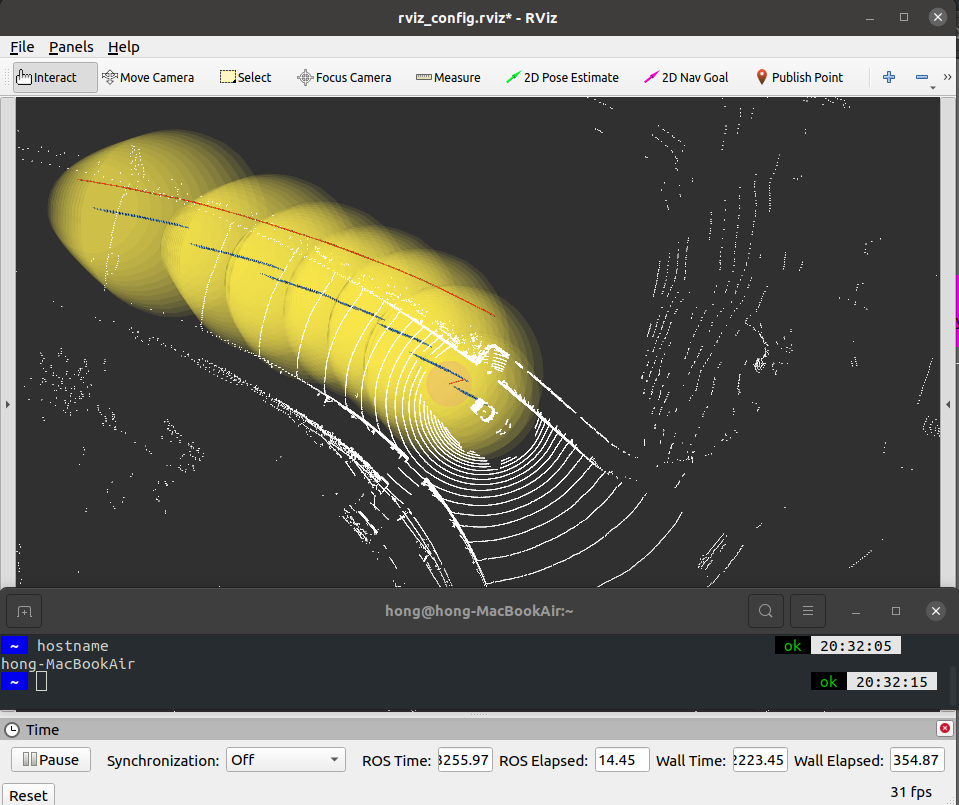
\includegraphics[scale=0.35]{predict_3.png}
	\caption{動態估測Rviz}
	\label{fig:1}
\end{center}
\end{figure}
\begin{figure}[H]
	\centering
	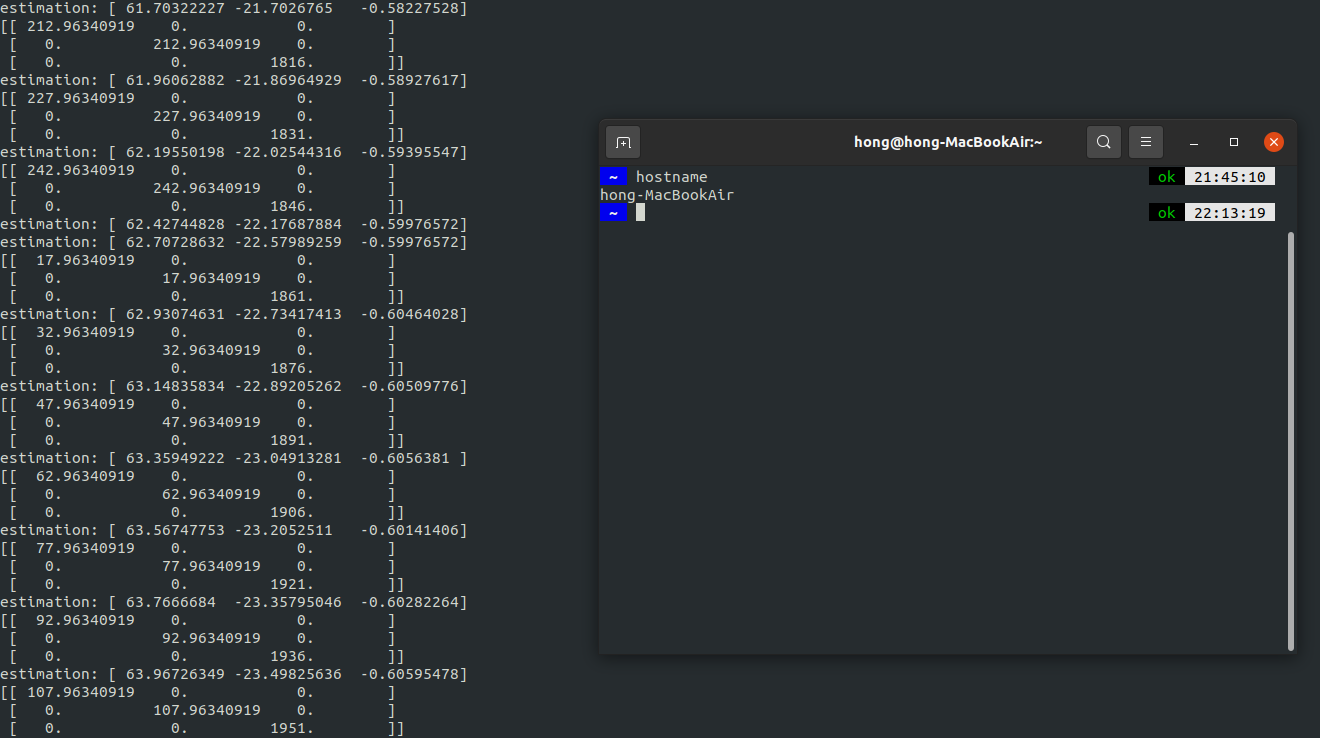
\includegraphics[scale=0.3]{./predict3.png}
	\caption{Predict [ x y yaw ] 三維度P矩陣}
\end{figure}
\begin{figure}[H]
	\centering
	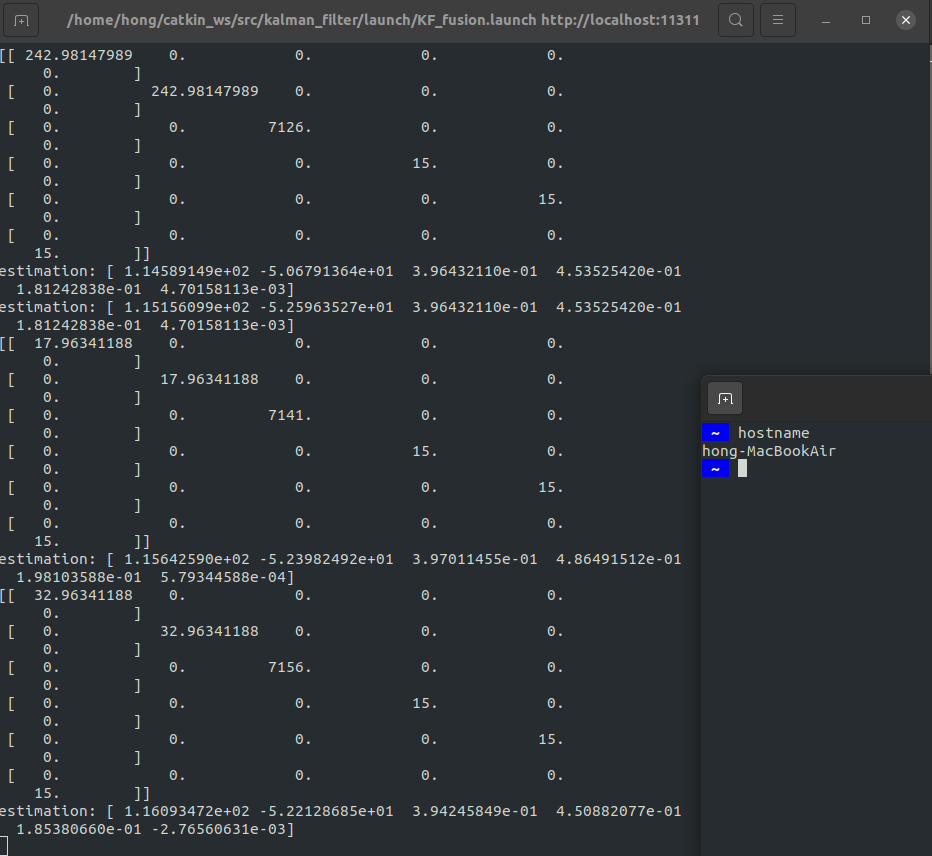
\includegraphics[scale=0.3]{./predict6.png}
	\caption{Predict [ x y yaw $\Delta{x}$ $\Delta{y}$ $\Delta{yaw}$] 六維度狀態P矩陣}
\end{figure}


\begin{thebibliography}{1}
 
\bibitem{1}
    Labbe, R. (2014). Kalman and bayesian filters in python. Chap, 7(246), 4.
\end{thebibliography}

\end{document}
